\documentclass[tikz,border=2pt]{standalone}
\usepackage{amsmath,amssymb}
\usepackage{tikz}
\usetikzlibrary{arrows.meta}

\begin{document}
% The three reasons to stop exploring a branch-and-bound node (maximisation, incumbent L):
% its relaxation is infeasible, its relaxation is already integer, or its bound is <= L.
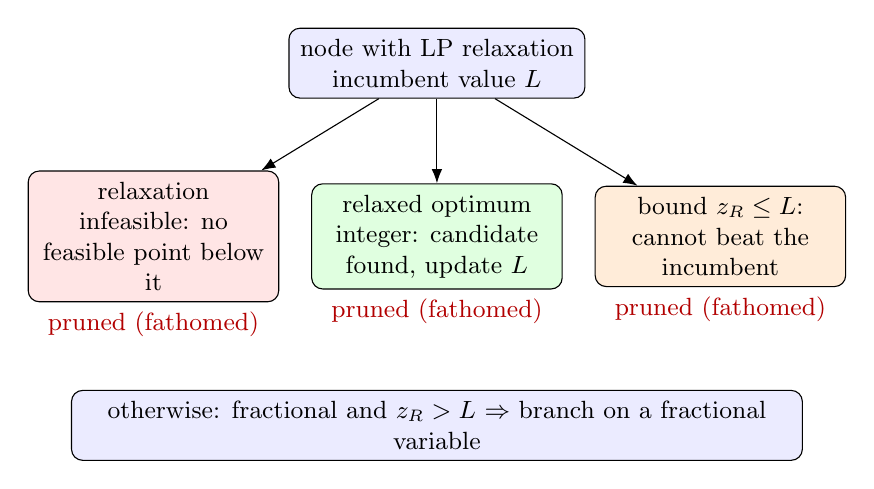
\begin{tikzpicture}[every node/.style={font=\small}, >={Latex[length=1.8mm]}, nd/.style={draw, rounded corners=4pt, inner sep=4pt, align=flush center}]
	\node[nd, fill=blue!8] (r) at (0,0) {node with LP relaxation\\ incumbent value $L$};
	\node[nd, fill=red!10, text width=2.9cm] (a) at (-3.6,-2.2) {relaxation infeasible: no feasible point below it};
	\node[nd, fill=green!12, text width=2.9cm] (b) at (0,-2.2) {relaxed optimum integer: candidate found, update $L$};
	\node[nd, fill=orange!15, text width=2.9cm] (c) at (3.6,-2.2) {bound $z_R\le L$: cannot beat the incumbent};
	\draw[->] (r) -- (a); \draw[->] (r) -- (b); \draw[->] (r) -- (c);
	\foreach \n in {a,b,c} {\node[red!70!black, anchor=north] at (\n.south) {pruned (fathomed)};}
	\node[nd, fill=blue!8, text width=9cm] (d) at (0,-4.6) {otherwise: fractional and $z_R>L$ $\Rightarrow$ branch on a fractional variable};
	\end{tikzpicture}
\end{document}
